\section{Architecture générale}
Le but du projet est de permettre à des applications de modifier des fichiers stockés à différents endroits, via le protocole défini par Ubuntu One.\\

Pour cela, plusieurs composants sont nécessaires :
\begin{itemize} 
   \item Le serveur : Le serveur reçoit des instructions via l'API d'Ubuntu One, par HTTP.
   \item Les clients : Les clients sont la partie utilisateur. Ces clients échangent avec le serveur via l'API. 
   \item Les drivers : Les drivers permettent d'échanger entre le serveur et les différentes solutions de stockage. 
\end{itemize}

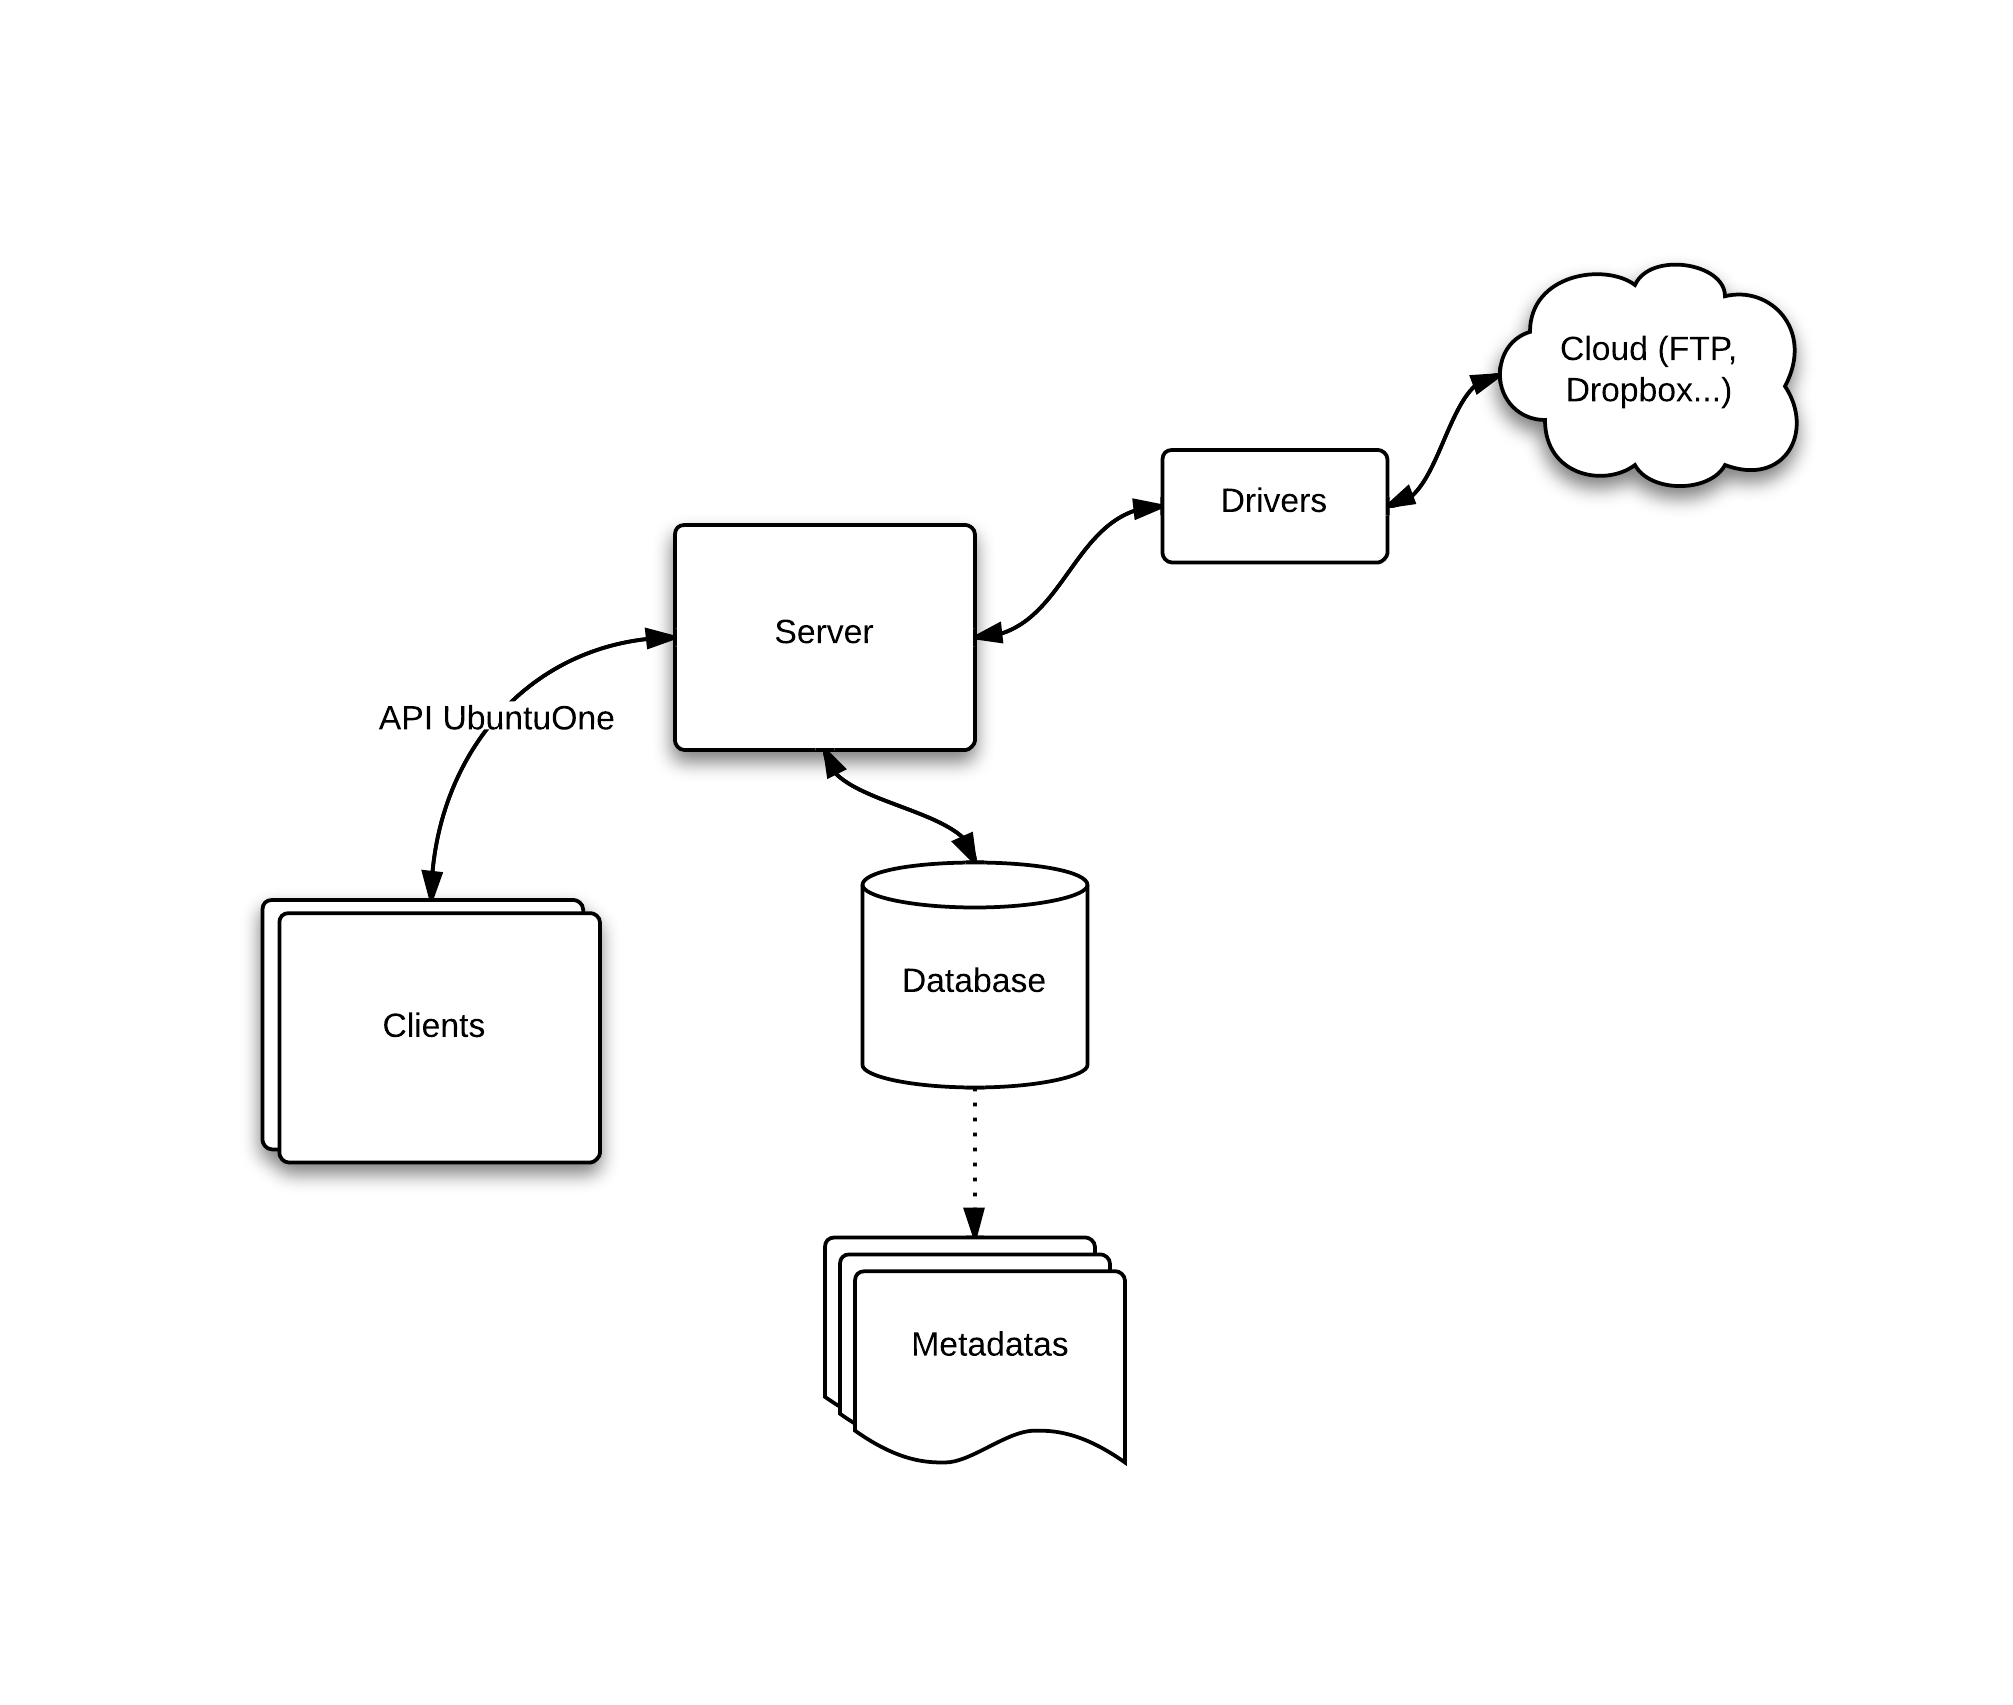
\includegraphics[width=500pt]{architecture.png}

\section{Serveur}
Le serveur est la partie centrale du projet. Il doit interpréter les instructions envoyées par les clients, et y répondre.\\

Une implémentation a été effectuée par l'entreprise Canonical, à l'origine d'Ubuntu One. Cette implémentation utilise les services de Cloud Computing EC2 et S3 d'Amazon. Suite à un partenariat entre ces deux entreprises, le code source du serveur n'est pas disponible, et ne le sera a priori jamais.\\

Onitu permet aux utilisateurs de choisir plusieurs moyens pour stocker leur données. Du point de vue du serveur, cela se fait grâce aux méta-données stockées en base de données, qui contiennent les informations nécessaires aux drivers pour récupérer les données.\\

\section{Drivers}
Les drivers permettent la communication entre le serveur et les différentes solutions de stockage. Ils sont construits autour d'une interface commune, qu'ils étendent afin d'interagir avec la solution à laquelle ils sont destinés.\\

Tous les drivers doivent permettre d'effectuer les quatre opérations de base : la création d'un fichier, sa récupération, son édition et sa suppression (connu sous l'acronyme CRUD, pour Create, Read, Update, Delete).\\

Du fait du côté ouvert d'Onitu, n'importe qui peut créer son propre Driver. Ceci dit, plusieurs sont prévus et seront maintenus dans le cadre de l'EIP :
\begin{itemize}
    \item Stockage local : Pour permettre de stocker des fichiers sur le serveur où est installé Onitu.
    \item Dropbox/Box.com/Google Drive/SkyDrive : Onitu peut utiliser ces services tiers pour récupérer et stocker les fichiers, si l'utilisateur y possède un compte.
    \item (S)FTP/SSH/NFS/Webdav/Samba/HTTP : Des drivers permettent d'utiliser n'importe quel serveur supportant au moins un de ces protocoles. Cela permet à un utilisateur d'étendre simplement son espace de stockage sans être dépendant d'un service qu'il ne maîtrise pas.
    \item Amazon S3 : Onitu est compatible avec la solution de stockage dans le cloud d'Amazon, une des plus utilisée au monde.
    \item OwnCloud : OwnCloud est un service relativement similaire à Onitu, il est donc intéressant de pouvoir interagir avec lui.
    \item Ubuntu One : Il est possible d'utiliser n'importe quel serveur compatible avec l'API d'Ubuntu One comme serveur de stockage, c'est à dire un autre serveur Onitu ou bien le serveur officiel de Canonical.
\end{itemize}

\section{Base de données}
Les meta-données liées au fichiers seront stockées dans une base de données, au sein du serveur. La majeur partie de ces métas-données est définie par le protocole d'Ubuntu One.\\

Onitu étends ces métas-données afin d'ajouter les informations nécessaires aux Drivers. La forme de ces informations est, dans l'ensemble, laissée libre à chaque Driver.\\

Cette flexibilité est rendue possible grâce à l'utilisation d'une base de type NoSQL orientée document, MongoDB.

\section{Clients}
Des clients existent déjà pour Ubuntu One, sur de nombreuses plateformes (Linux, Windows, Mac OS, Android, iOS). Onitu étant entièrement compatible avec l'API d'Ubuntu One, ces clients peuvent interagir avec lui.\\

Cependant, la plupart des clients ne permettent pas de choisir l'adresse du serveur, étant donné que pour le moment un seul serveur de référence existe. Il est donc prévu d'intégrer la possibilité de changer le serveur dans les différents clients.\\

Le but d'Onitu n'est pas de fournir des clients, mais un serveur. Des clients pourraient tout de même être développés par l'équipe en parallèle, à des fins de tests, ou bien afin d'offrir un pannel plus complet aux utilisateurs. Un client utilisant FUSE, une bibliothèque permettant de créer des systèmes de fichiers, est notamment envisagé.\\

\section{Interface Web}
Actuellement, Ubuntu One propose une interface web, hébergée sur le service Amazon EC2. Cette interface fait partie du serveur, et les sources ne sont donc pas publiques.
Onitu se doit donc de remplacer cette interface web.\\

L'interface web est destinée aux utilisateurs ayant des droits suffisants pour accéder à certains dossiers, ainsi qu'à l'administrateur qui peut effectuer la plupart des actions de configuration sur cette interface.\\

L'interface web dispose de plusieurs fonctionnalités :
\begin{itemize}
    \item Charger de nouveaux fichiers
    \item Éditer les dossiers et les noms de fichiers
    \item Éditer les fichiers textes de manière simple
    \item Télécharger des fichiers
    \item Éditer les droits liés au partage des fichiers
    \item Ajouter, supprimer ou modifier les options liées aux services externes, qui communiquent par le biais des Drivers
    \item Éditer les différentes options de configuration du serveur
\end{itemize}